%\section{Data and Analysis}

The \minerva detector was exposed to the NuMI neutrino beam at Fermilab, configured for this analysis to produce a beam consisting of $>95\%$ $\nu_\mu$ at the peak energy of 3~GeV. The neutrino flux is predicted 
using a Geant4-based simulation tuned to hadron production 
data~\cite{Alt:2006fr} as described in Ref.~\cite{nubarprl}.
This analysis uses data taken between March and July 2010 with
$9.42\times 10^{19}$ protons on target.

The \minerva detector consists of a fine-grained scintillator tracker
surrounded by electromagnetic and hadronic 
calorimeters\footnote{The \minerva scintillator tracking region is 95\% CH and 5\% other materials by weight.}~\cite{minerva_nim}. The detector enables 
reconstruction of the neutrino interaction point, 
the tracks of outgoing charged particles, 
and the calorimetric reconstruction of other particles produced in the interaction. 
\minerva is located \unit[2]{m} upstream of the 
MINOS near detector~\cite{Michael:2008bc}, which is used to 
reconstruct the momentum and charge of muons.
The hadronic energy scale is set
using data from through-going muons and a scaled down 
\minerva detector exposed to a hadron test beam~\cite{minerva_nim}.  
The detector's performance is simulated by a Geant4-based hit-level 
simulation and a readout model tuned to match the data~\cite{minerva_nim}.   
Event pile-up causes a decrease in the muon track reconstruction efficiency 
which we studied in both \minerva and \minos by projecting tracks 
found in one of the detectors to the other 
and measuring the misreconstruction rate. 
This resulted in a -9.1\% (-4.8\%) correction to the simulated 
efficiency for muons with momenta below (above) 3 GeV/c in MINOS.
Neutrino interactions in the detector are simulated using the 
GENIE neutrino event generator~\cite{Andreopoulos201087}.  Details of the cross section models and associated parameters are described in
Ref.~\cite{nubarprl}.  

Event reconstruction and selection for this analysis is nearly identical
to that used in the \minerva antineutrino quasi-elastic
measurement~\cite{nubarprl} with small modifications to account for
the likelihood of a leading proton in the final state instead of a neutron.  
We require events to have a $\mu^-$ originating in the 
\unit[5.57]{metric ton} fiducial volume and assign remaining clusters with 
energies $>\unit[1]{MeV}$ to the recoiling hadronic system. 
The aforementioned vertex region corresponds to a sphere with
$\unit[30]{g/cm^2}$ of material centered on the vertex. 
The recoil system outside the vertex region is required to have $\leq 2$ isolated groups of spatially contiguous energy depositions\footnote{Isolated energy depositions are created directly by the leading proton or by secondary hadronic interactions in the detector.}.

The neutrino energy and the square of the four momentum transferred to the
nucleus, $Q^2_{QE}$, are estimated from the muon momentum and 
angle using a quasi-elastic hypothesis, as in the antineutrino
analysis~\cite{nubarprl}.  The binding energy correction is taken to be 
\unit[+34]{MeV} instead of \unit[+30]{MeV} used in Ref.~\cite{nubarprl} due to
Coulomb corrections~\cite{Katori:2008zz}, 
and the proton and neutron masses are interchanged.

\begin{figure}[tp]
\centering
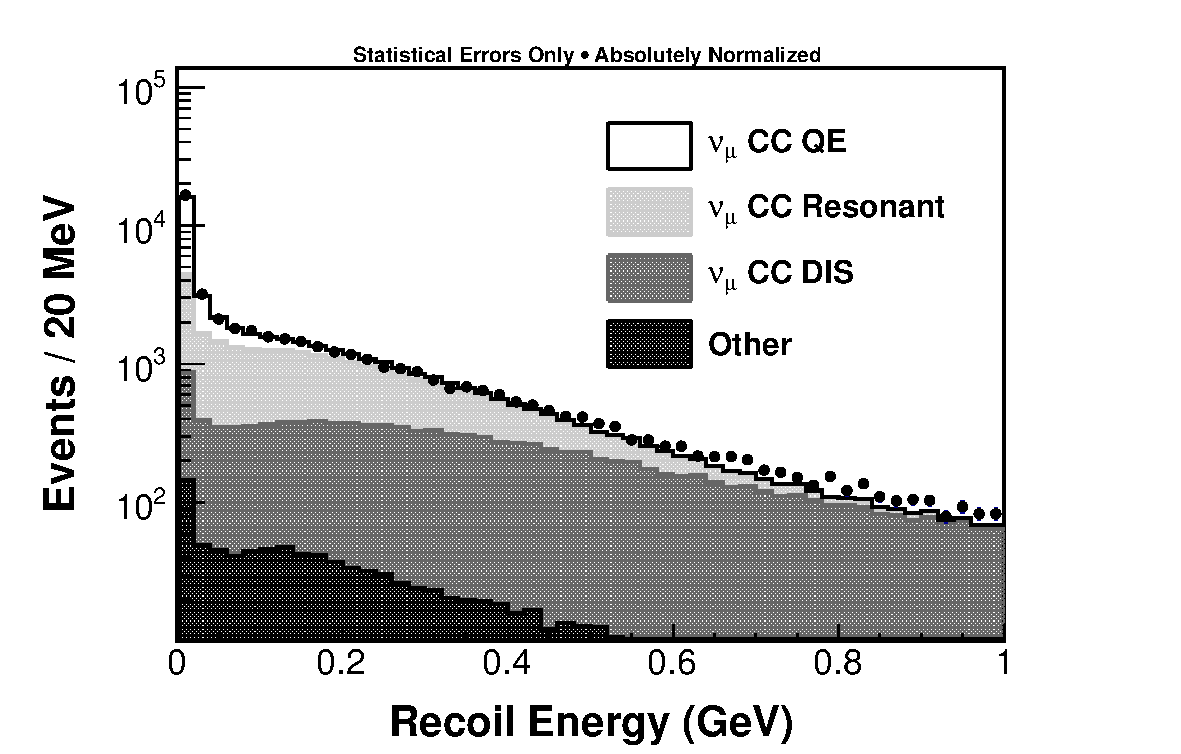
\includegraphics[width=\columnwidth]{figures/Figure1_nu}
\caption{\label{fig:recoil} The measured recoil energy distribution in the data (solid circles) and the predicted composition of signal and background. Backgrounds from baryon resonance production (light grey), continuum/deep-inelastic scattering (dark grey), and other sources (black), such as coherent pion production, are shown.  The fraction of signal before requiring low recoil energy is $0.29$.}
\end{figure}
\begin{figure}[tp]
\centering
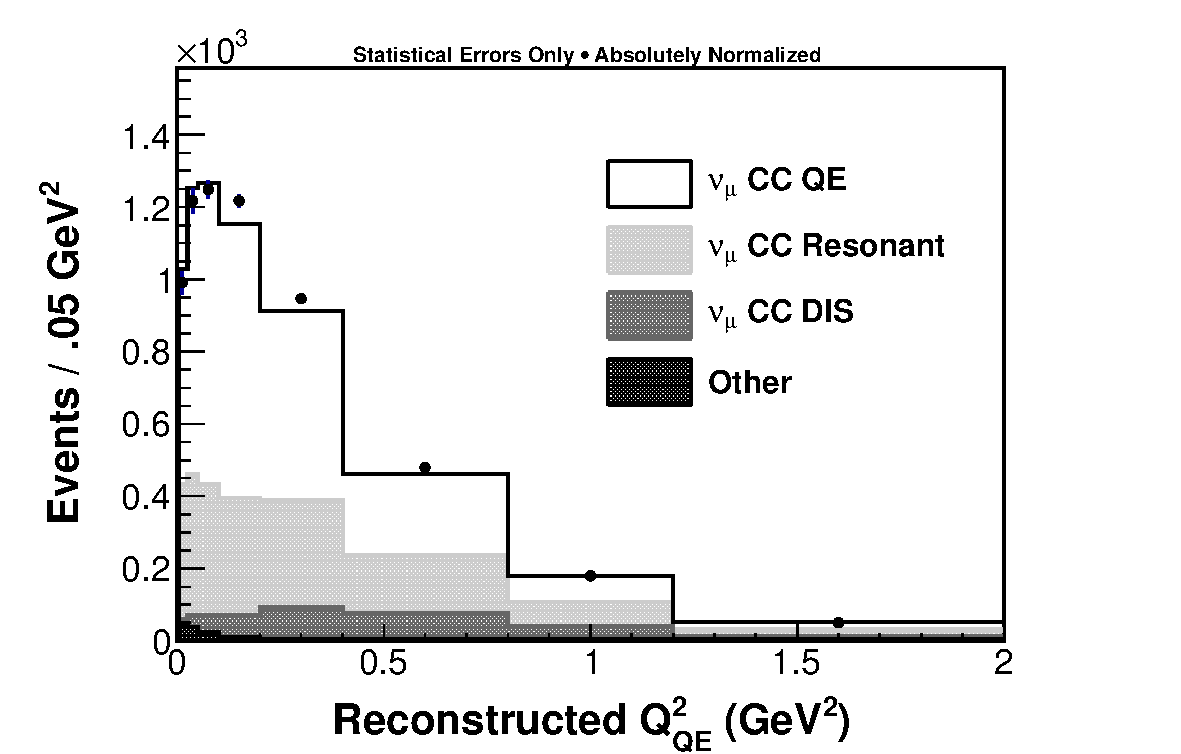
\includegraphics[width=\columnwidth]{figures/Figure2_nu}
\caption{The measured $Q^2_{QE}$ distributions in the data and the simulation, before correcting for detector resolution and acceptance.   The fraction of signal in this sample is $0.49$, and 47\% of signal events in our fiducial volume pass all selections.}
\label{fig:qsq}
\end{figure}

Figure~\ref{fig:recoil} shows that the quasi-elastic signal
preferentially populates lower recoil energies.  However, since the proton's kinetic energy is $\approx Q^2/2M_\text{neutron}$ for quasi-elastic scattering, the recoil 
energy is expected to scale with the momentum transfer as the 
final state proton becomes increasingly energetic and escapes the vertex region.
We account for this by varying a cut on the maximum 
allowed recoil energy as a function of \Qsqqe to assure 
95\% signal efficiency in each  \Qsqqe bin.  

The background in each $Q^2_{QE}$ bin is estimated from the data by fitting the relative normalizations of signal and background recoil energy distributions whose shapes are taken from the simulation.   This procedure reduces the relative background prediction by 15\% below $Q^2_{QE}$ of 0.8~GeV$^2$ and 5\% between 0.8 and 2.0~GeV$^2$.  The purity of the resulting sample 
ranges from 65\% at low \Qsqqe to 40\% at higher \Qsqqe.
Figure \ref{fig:qsq} compares the \Qsqqe distribution 
of the 29,620 events which satisfy the selection criteria to 
the simulation after rescaling the background according to the fit.
The cross-section as a function of \Qsqqe is extracted by subtracting the backgrounds, correcting for detector resolution and acceptance, and dividing by the number of neutrons in the fiducial volume ($1.65 \pm 0.02 \times 10^{30}$) and by the flux, as described in Ref.~\cite{nubarprl}.  The total neutrino 
flux integrated between 1.5 and 10~GeV is estimated by the simulation to be 
$2.91\times 10^{-8}/$cm$^2$ per proton on target\footnoteremember{footsupp}{See Supplemental Material\ SuppLocation\ for the flux as a function of energy and for correlations of uncertainties among bins for the cross-section and shape measurement.}.

The same systematic uncertainties which affect the antineutrino
analysis~\cite{nubarprl} are evaluated in this analysis.  
Table~\ref{tab:systematics} shows a summary of
systematic uncertainties on $d\sigma/dQ^2_{QE}$. 
The largest uncertainties on the absolute cross-section 
come from the neutrino flux and the muon momentum scale.  
However, the flux uncertainty is largely independent of $Q^2_{QE}$ so comparisons of the shape of $d\sigma/dQ^2_{QE}$  to scattering model predictions are relatively insensitive to knowledge of the flux. 
The saturation of ionization ($dE/dx$), parameterized by Birk's law and characterized by a factor of $(1 + k_B\times dE/dx)^{-1}$, leads to a recoil reconstruction uncertainty; this uncertainty is negligible for the antineutrino $d\sigma/dQ^2_{QE}$ measurement but is important for the neutrino measurement.
By studying stopping proton tracks in the \minerva test beam detector
we estimate $k_B=\unit[0.13\pm0.04]{mm/MeV}$~\cite{minerva_nim}, and vary
the ionization accordingly in the simulation to propagate the uncertainty.

%\begin{figure}[tp]
%\centering
%\includegraphics[width=75mm, trim=2cm 0cm 2cm 0cm]{figures/err_summary_total_bayes_variedbackgrounds_fit_sometimesUnsmeared_standard_minervanu}
%\caption{\label{fig:syst_err} Systematic uncertainty summary for the 
%cross-section measurement as a function of $Q^2_{QE}$.}
%\end{figure}

\begingroup
\squeezetable
\begin{table}
\begin{tabular}{cccccccc}
$Q^2_{QE}$ (GeV$^2$) & I & II & III & IV & V & VI & Total \\
\hline
$0.0 - 0.025$ & 0.06 & 0.04 & 0.02 & 0.04 & 0.09 & 0.03 & 0.13 \\
$0.025 - 0.05$ & 0.06 & 0.03 & 0.02 & 0.03 & 0.09 & 0.02 & 0.12 \\
$0.05 - 0.1$ & 0.06 & 0.03 & 0.02 & 0.03 & 0.09 & 0.02 & 0.12 \\
$0.1 - 0.2$ & 0.06 & 0.03 & 0.03 & 0.02 & 0.09 & 0.02 & 0.11 \\
$0.2 - 0.4$ & 0.05 & 0.02 & 0.03 & 0.03 & 0.09 & 0.01 & 0.11 \\
$0.4 - 0.8$ & 0.05 & 0.03 & 0.04 & 0.04 & 0.09 & 0.01 & 0.13 \\
$0.8 - 1.2$ & 0.08 & 0.07 & 0.07 & 0.15 & 0.09 & 0.02 & 0.22 \\
$1.2 - 2.0$ & 0.12 & 0.07 & 0.07 & 0.16 & 0.09 & 0.02 & 0.24 \\
\hline
\end{tabular}
\caption{
Fractional systematic uncertainties on $d\sigma/dQ^2_{QE}$ associated with (I) muon reconstruction, (II) recoil reconstruction, (III) neutrino interaction models, (IV) final state interactions, (V) flux and (VI) other sources.  
The rightmost column shows the total fractional systematic uncertainty due to all sources.
}
\label{tab:systematics}
\end{table}
\endgroup


The vertex energy distribution is sensitive to the multiplicity of low energy charged hadrons in the final state. 
%multi-nucleon effects, therefore and 
Systematic uncertainties on this distribution are evaluated with the same methods 
used for the cross-section measurement.  The largest uncertainties in the
distribution come from the detector's response to protons (constrained by test beam measurements~\cite{minerva_nim}), the Birk's law constant discussed above, and GENIE's final state interactions model.  The latter is evaluated by varying the underlying model tuning parameters within their systematic uncertainties.
